\documentclass[aspectratio=169]{../latex_main/tntbeamer}  % you can pass all options of the beamer class, e.g., 'handout' or 'aspectratio=43'
\usepackage{dsfont}
\usepackage{bm}
\usepackage[english]{babel}
\usepackage[T1]{fontenc}
%\usepackage[utf8]{inputenc}
\usepackage{graphicx}
\graphicspath{ {./figures/} }
\usepackage{algorithm}
\usepackage[ruled,vlined,algo2e,linesnumbered]{algorithm2e}
\usepackage{hyperref}
\usepackage{booktabs}
\usepackage{mathtools}

\usepackage{amsmath,amssymb}

\DeclareMathOperator*{\argmax}{arg\,max}
\DeclareMathOperator*{\argmin}{arg\,min}

\usepackage{amsbsy}
\newcommand{\vect}[1]{\bm{#1}}
%\newcommand{\vect}[1]{\boldsymbol{#1}}

\usepackage{pgfplots}
\pgfplotsset{compat=1.16}
\usepackage{tikz}
\usetikzlibrary{trees} 
\usetikzlibrary{shapes.geometric}
\usetikzlibrary{positioning,shapes,shadows,arrows,calc,mindmap}
\usetikzlibrary{positioning,fadings,through}
\usetikzlibrary{decorations.pathreplacing}
\usetikzlibrary{intersections}
\pgfdeclarelayer{background}
\pgfdeclarelayer{foreground}
\pgfsetlayers{background,main,foreground}
\tikzstyle{activity}=[rectangle, draw=black, rounded corners, text centered, text width=8em]
\tikzstyle{data}=[rectangle, draw=black, text centered, text width=8em]
\tikzstyle{myarrow}=[->, thick, draw=black]

% Define the layers to draw the diagram
\pgfdeclarelayer{background}
\pgfdeclarelayer{foreground}
\pgfsetlayers{background,main,foreground}

% Requires XeLaTeX or LuaLaTeX
%\usepackage{unicode-math}

\usepackage{fontspec}
%\setsansfont{Arial}
\setsansfont{RotisSansSerifStd}[ 
Path=../latex_main/fonts/,
Extension = .otf,
UprightFont = *-Regular,  % or *-Light
BoldFont = *-ExtraBold,  % or *-Bold
ItalicFont = *-Italic
]
\setmonofont{Cascadia Mono}[
Scale=0.8
]

% scale factor adapted; mathrm font added (Benjamin Spitschan @TNT, 2021-06-01)
%\setmathfont[Scale=1.05]{Libertinus Math}
%\setmathrm[Scale=1.05]{Libertinus Math}

% other available math fonts are (not exhaustive)
% Latin Modern Math
% XITS Math
% Libertinus Math
% Asana Math
% Fira Math
% TeX Gyre Pagella Math
% TeX Gyre Bonum Math
% TeX Gyre Schola Math
% TeX Gyre Termes Math

% Literature References
\newcommand{\lit}[2]{\href{#2}{\footnotesize\color{black!60}[#1]}}

%%% Beamer Customization
%----------------------------------------------------------------------
% (Don't) Show sections in frame header. Options: 'sections', 'sections light', empty
\setbeamertemplate{headline}{empty}

% Add header logo for normal frames
\setheaderimage{
	% 
\includegraphics[height=\logoheight]{figures/TNT_darkv4.pdf}
	
\includegraphics[height=\logoheight]{../latex_main/figures/luh_logo_rgb_0_80_155.pdf}
	% 
\includegraphics[height=\logoheight]{figures/logo_tntluh.pdf}
}

% Header logo for title page
\settitleheaderimage{
	% 
\includegraphics[height=\logoheight]{figures/TNT_darkv4.pdf}
	
\includegraphics[height=\logoheight]{../latex_main/figures/luh_logo_rgb_0_80_155.pdf}
	% 
\includegraphics[height=\logoheight]{figures/logo_tntluh.pdf}
}

% Title page: tntdefault 
\setbeamertemplate{title page}[tntdefault]  % or luhstyle
% Add optional title image here
%\addtitlepageimagedefault{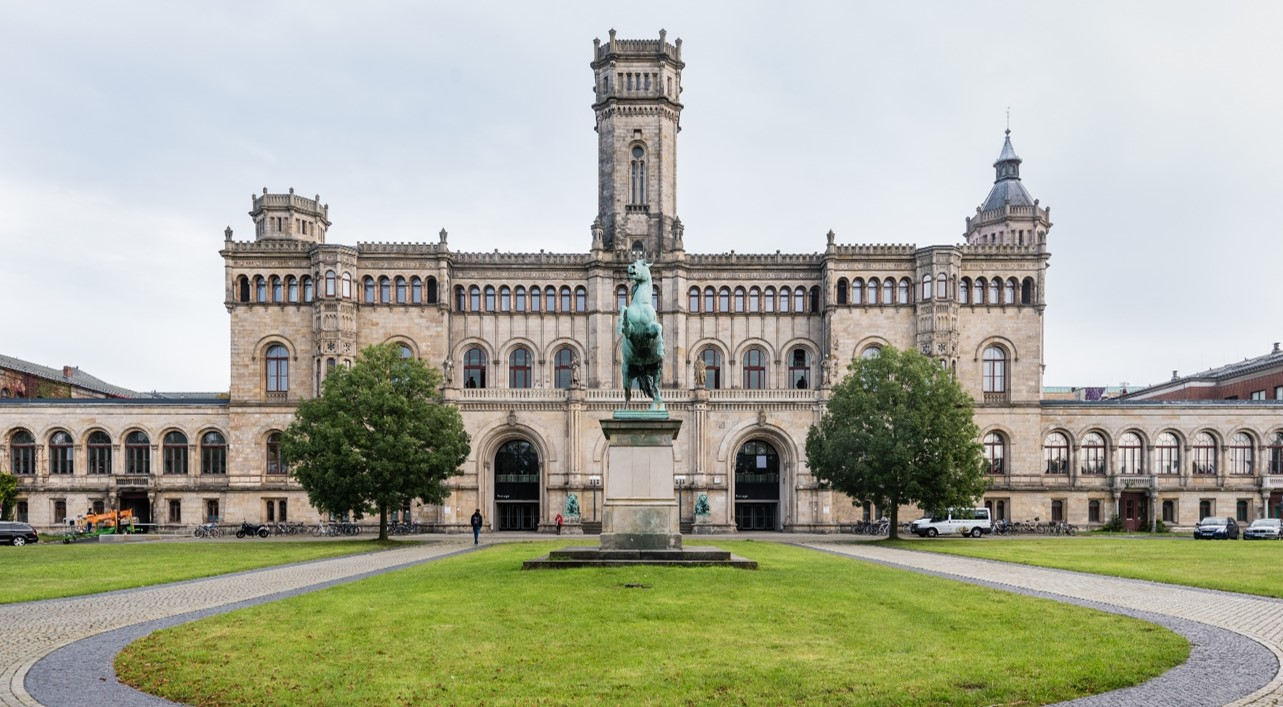
\includegraphics[width=0.65\textwidth]{figures/luh_default_presentation_title_image.jpg}}

% Title page: luhstyle
% \setbeamertemplate{title page}[luhstyle]
% % Add optional title image here
% \addtitlepageimage{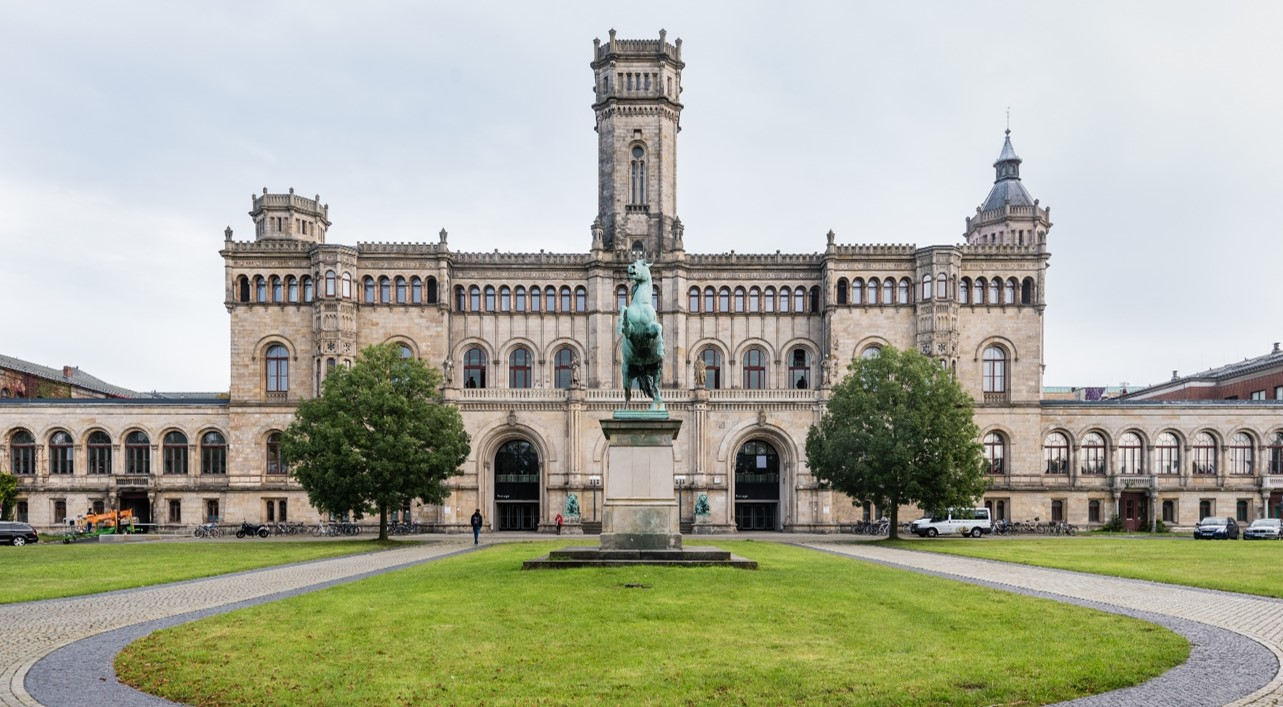
\includegraphics[width=0.75\textwidth]{figures/luh_default_presentation_title_image.jpg}}

\author[Abedjan \& Lindauer]{Ziawasch Abedjan \& Marius Lindauer\\[1em]
	
\includegraphics[height=\logoheight]{../latex_main/figures/luh_logo_rgb_0_80_155.pdf}\qquad
	
\includegraphics[height=\logoheight]{../latex_main/figures/DBIS_Kurzlogo.png}\qquad

\includegraphics[height=\logoheight]{../latex_main/figures/TNT_darkv4}\qquad

\includegraphics[height=\logoheight]{../latex_main/figures/L3S.jpg}	}
\date{Summer Term 2022; \hspace{0.5em} {
\includegraphics[height=1.5em]{../latex_main/figures/Cc-by-nc-sa_icon.svg.png}}; based on \href{https://ds100.org/fa21/}{[DS100]}
}


%%% Custom Packages
%----------------------------------------------------------------------
% Create dummy content
\usepackage{blindtext}

% Adds a frame with the current page layout. Just call \layout inside of a frame.
\usepackage{layout}


%%% Macros
%\renewcommand{\vec}[1]{\mathbf{#1}}
% \usepackage{bm}
%\let\vecb\bm

\title[Reinforcement Learning]{DS: Learning}
\subtitle{Reinforcement Learning}

\graphicspath{ {./figure/} }
%\institute{}


\begin{document}
	
    \maketitle
    
    \begin{frame}{What is Reinforcement Learning?}

        \begin{itemize}
            \item At the beginning, we have \alert{no} data
            \item By interacting with the environment (e.g., a game or the real world discovered by a robot), we collect data in the form of $s_t, a_t, r_t, s_{t+1}$
            \begin{itemize}
                \item $s_t$ being the current state
                \item $a_t$ being the chosen action by the agent (e.g., robot)
                \item $r_t$ being the reward by choosing $a_t$ in $s_t$
                \item $s_{t+1}$ being the successor state after performing $a_t$ in $s_t$
            \end{itemize}
        \end{itemize}

        \centering
        \tikzstyle{activity}=[rectangle, draw=black, rounded corners, text centered, text width=6em, fill=white, drop shadow]
        \tikzstyle{data}=[rectangle, draw=black, text centered, fill=black!10, text width=6em, drop shadow]
        \tikzstyle{myarrow}=[->, thick]
        
        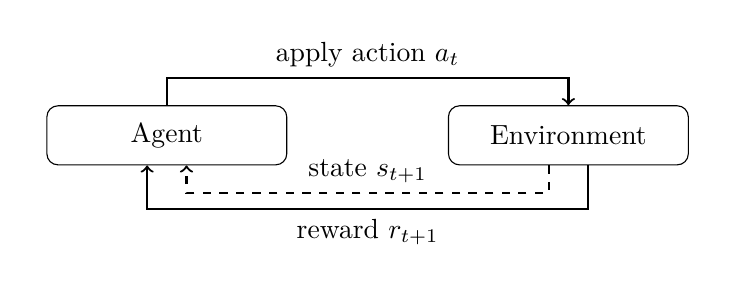
\begin{tikzpicture}[node distance=2.1cm]
        %PreProcessing
        
        \node (Agent) [activity,
        minimum height=.75cm] {Agent};
        
        \node (Algo) [activity, right of=Agent, xshift=3cm,
        minimum height=.75cm] {Environment};
        
        \begin{pgfonlayer}{background}
        \path (Agent -| Agent.west)+(-0.12,1.25) node (resUL) {};
        \path (Algo.east |- Algo.south)+(0.125,-1.25) node (resBR) {};
        
        % Context
        %\path [rounded corners, draw=black!50, fill=white] ($(resUL)+(0.5, -0.5)$) rectangle ($(resBR)+(0.5, -0.5)$);
        %\path [rounded corners, draw=black!50, fill=white] ($(resUL)+(0.375, -0.375)$) rectangle ($(resBR)+(0.375, -0.375)$);
        %\path [rounded corners, draw=black!50, fill=white] ($(resUL)+(0.25, -0.25)$) rectangle ($(resBR)+(0.25, -0.25)$);
        %\path [rounded corners, draw=black!50, fill=white] ($(resUL)+(0.125, -0.125)$) rectangle ($(resBR)+(0.125, -0.125)$);
        
        % Top level
        %\path [rounded corners, draw=black!50, fill=white] (resUL) rectangle (resBR);
        %\path (resBR)+(-.9,0.175) node [text=black!75] {instance $i$};
        %\path (resUL.east |- resBR.north)+(+.9,0.075) node [text=black!75] {control of $h$};
        
        \end{pgfonlayer}
        
        %        \draw[myarrow] (feat.south) -- ($(feat.south |- Agent)+(0,1.125)$);
        
        \draw[myarrow] (Agent.north) -- ($(Agent.north)+(0.0,+0.35)$) -- ($(Algo.north)+(0.0,+0.35)$) node [above,pos=0.5] {apply action $a_t$} node [below,pos=0.5] {} -- (Algo.north);
        \draw[myarrow, dashed] ($(Algo.south)+(-0.25, 0)$) -- ($(Algo.south)+(-0.25, -0.35)$) -- ($(Agent.south)+(0.25, -0.35)$) node [above,pos=0.5] {state $s_{t+1}$} -- ($(Agent.south)+(0.25, 0)$);
        \draw[myarrow] ($(Algo.south)+(0.25, 0)$) -- ($(Algo.south)+(0.25, -0.55)$) -- ($(Agent.south)+(-0.25, -0.55)$) node [below,pos=0.5] {reward $r_{t+1}$} -- ($(Agent.south)+(-0.25, 0)$);
        
        %\draw[<->, thick, draw=black!32.5] (resBR.east |- resUL.center) -- ($(resBR.east |- resUL.center)+(0.5, -0.5)$);
        
        \end{tikzpicture}

    \end{frame}

    \begin{frame}[c]{Markov Decision Process (MDP)}
    
    \begin{itemize}
    	\item Definition:
    	\begin{itemize}
    		\item $S$ is a (finite) set of Markov states $s \in S$
    		\item $A$ is a (finite) set of actions $a \in A$
    		\item $P$ is the dynamics/transition model for each action, that specifies $P(s_{t+1} = s' \mid s_t=s, a_t=a)$
    		\item $R$ is a reward function 
    		$R(s_t=s, a_t=a) = \mathbb{E}[r_t \mid s_t=s, a_t=a] $
    		\begin{itemize}
    			\item Sometimes R is also defined based on $(s)$ or on $(s,a,s')$
    		\end{itemize}
    		\item Discount factor $\gamma \in [0, 1]$
    	\end{itemize}
    	\item MDP is tuple $(S,A,P, R, \gamma)$
            \medskip
            \pause
            \item \alert{Goal}: finding an optimal policy $\pi: s_t \mapsto a_t$
            $$ \pi^*(s)  \in \argmax_\pi V^\pi(s)$$
            with 
            $$V^\pi (s) &=& \mathbb{E}_\pi [r_t + \gamma V_{k-1} \mid s_t = s] $$
            
            
    \end{itemize}
    
    \end{frame}
    %-----------------------------------------------------------------------
       

    \begin{frame}{Q-Learning}

        \begin{itemize}
            \item Let's consider our actions chosen by $\pi$ explicitly
            $$V^{\pi_i}(s) = \sum_{a \in A} \pi_i(a|s) Q^{\pi_i}(s,a)$$
            \pause
            \item If we can learn the state-action value function $Q$, we can choose the optimal action
            $$\pi(s) &\in& \argmax_{a \in A} Q(s,a)$$
            \item We learn $Q$ iteratively by collecting experience $s_t, a_t, r_t, s_{t+1}$
            $$Q(s_t,a_t) &\gets& Q(s_t, a_t) + \alpha (r_t + \gamma \max_{a' \in A} Q(s_{t+1}, a') - Q(s_t, a_t))$$
        \end{itemize}
        
   \end{frame}

\end{document}